For the alloy part we focused on modelling the ranking of a tournament ($T$) and see how it evolves after groups submit their code.
We also analyse different properties of the ranking ($R_{t,T}$) a relation that establishes which student ($s\in S$) ranks better or equal depending on their score and their current submissions($R_{t,T}\subseteq S\times S$).

\begin{lstlisting}[language=alloy]
open util/relation
open util/boolean


sig Tournament {}

//A battle has to belong to exactly one tournament
sig Battle {
	belongsTo: one Tournament
}

sig Student {}

//A group is a team of students for a specific battle
sig Group {
	participants: set Student,
	battle: Battle
} { participants !=none and cannotEnrollTwiceInABattle }

//We rename it for clarity
sig Score in Int {}
 
//The submission it is of a specific group and has associated a score
//To represent that submissions are submitted over time we added the submited attribute
sig Submission {
	group: one Group,
	score: one Score,
	var submited: one Bool
}{ score>=0 and score<=100 }
//Here we capture the fact that student can enroll only once to any battle if not it would be unfair
pred cannotEnrollTwiceInABattle {
	all disj g,h:Group | g.participants&h.participants=none or g.battle!=h.battle
}


//Auxiliary functions used to compute the score:

//Retrieves all the submissions of a group
fun submissions [g:Group]:set Submission{
	(group:>g).dom
}

//Retrieves only the submited ones of a group
fun effectiveSubmissions [g:Group]:set Submission{
	{s:g.submissions | s.submited.isTrue}
}

//Calculates all the obtained scores of a group until that moment
fun scores [g:Group]: set Score{
	g.effectiveSubmissions.score
}

//The best score of a group if it has not submitted it is 0
fun bestScore [g:Group]: Score {
	max[g.scores + {0}]
}

//The participants of a tournament in this case it is not necessary to have submitted jus to be enrolled (be part of a group in any of the battles belonging to it)
fun participants[t:Tournament]:Student {
	{s:Student | (some g:Group | t=g.battle.belongsTo and s in g.participants)}
}

//Score of the student only considering the scores obtained in the battles belonging to it
fun scoreInTournament[s:Student, t:Tournament]: Int{
	sum g:s.groupsForATournament[t] | g.bestScore
}

//For the prevoius we need to retrieve the groups in which the student participates related to the tournament
fun groupsForATournament[s:Student, t:Tournament]: set Group {
	{g:Group | s in g.participants and t=g.battle.belongsTo }
}

//Returns the ranking relation for a tournament as previously explained
fun ranking[t:Tournament]: Student -> Student {
	{b,w: t.participants | int b.scoreInTournament[t]>= int w.scoreInTournament[t]}
}


//To model correctly the evolution of the competition we add the following facts:

//The competition begins with 0 effective submissions
fact noSubmissionsAtStart {
		all s:Submission| s.submited.isFalse
}

//It ends after all the generated submissions become effective
pred allTournamentsEnd {
	eventually all s:Submission| s.submited.isTrue
}
fact {allTournamentsEnd}

//Each step can only submit one submission
pred submit [s:Submission]{
	submited' = submited ++ s->True
}
fact oneSubmissionPerStep {
	always some s:Submission| s.submit
}

\end{lstlisting}

\section{Examples}
\begin{figure}[h]
\caption{A simple example with two submissions to see if the behavior is the expected one}

\centering
\begin{lstlisting}[language=alloy]
run {} for 5 but exactly 2 Submission, 9 int
\end{lstlisting}

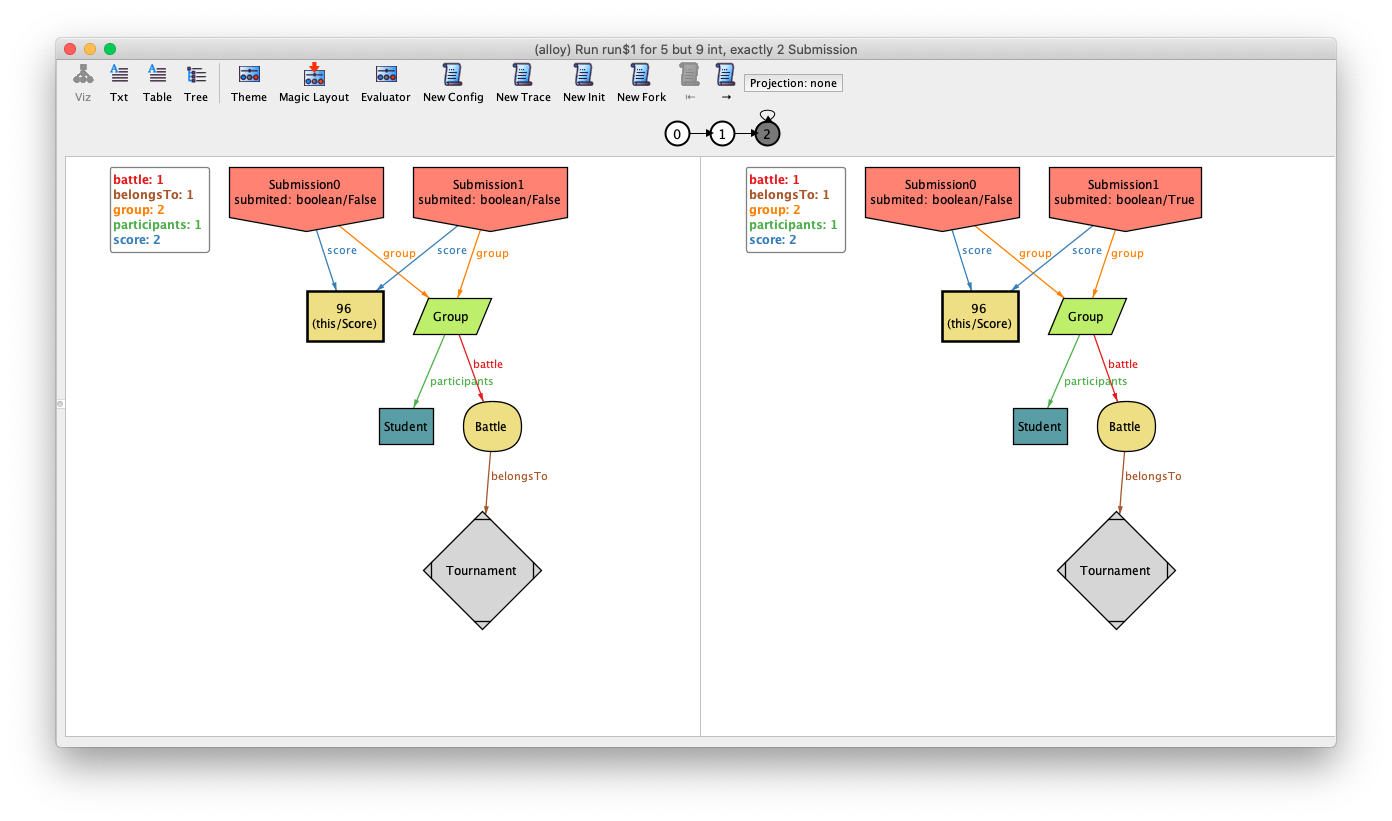
\includegraphics[width=\textwidth]{Images/First example 1.png}
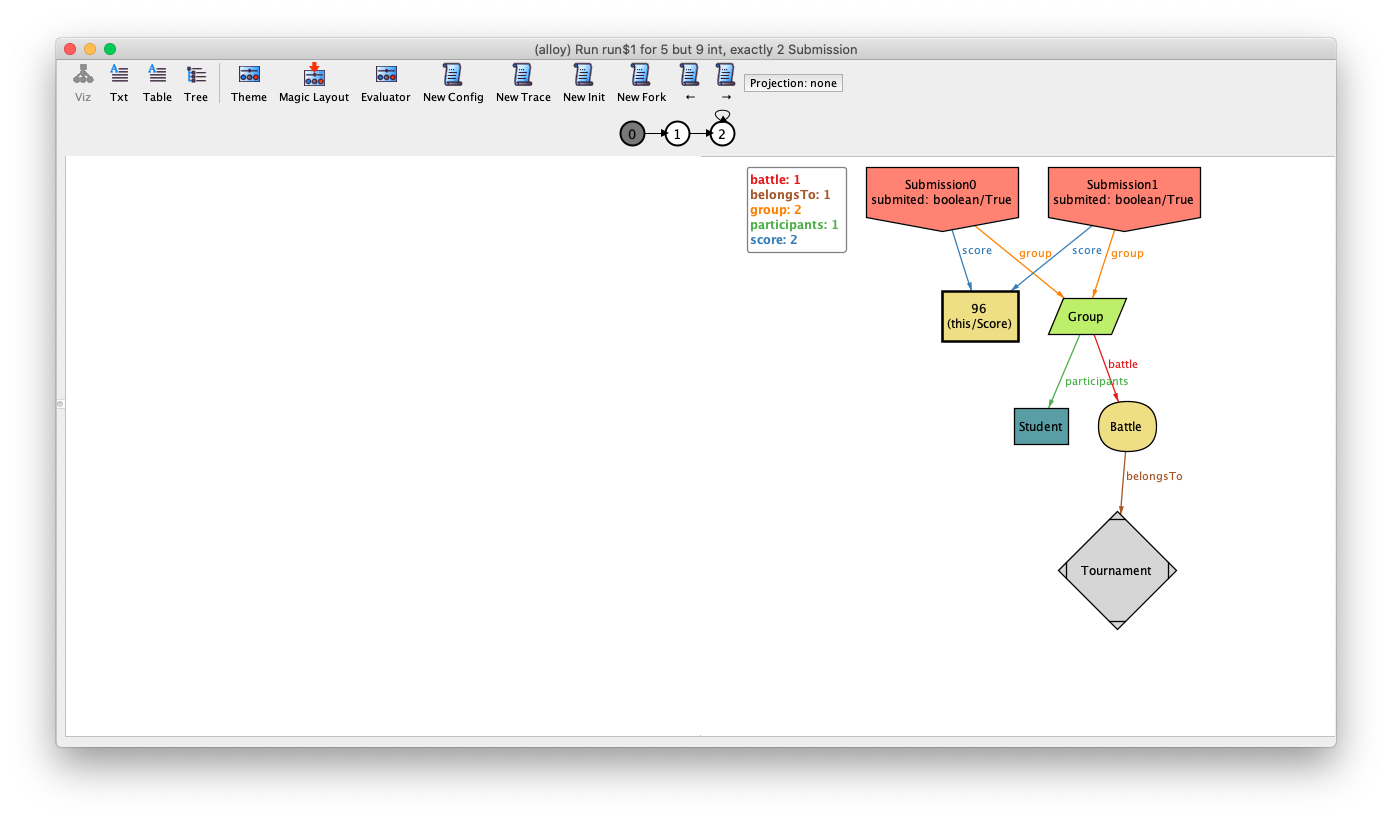
\includegraphics[width=\textwidth]{Images/First example 2.png}

\end{figure}

\begin{figure}[h]
\caption{An example where the final ranking is a relation of total order (i.e. with no ties and everyone participates)}

\centering
\begin{lstlisting}[language=alloy]
run {
	eventually some t:Tournament |  totalOrder[t.ranking,Student] 
} for 3 but exactly 1 Tournament, exactly 3 Student, 9 int
\end{lstlisting}

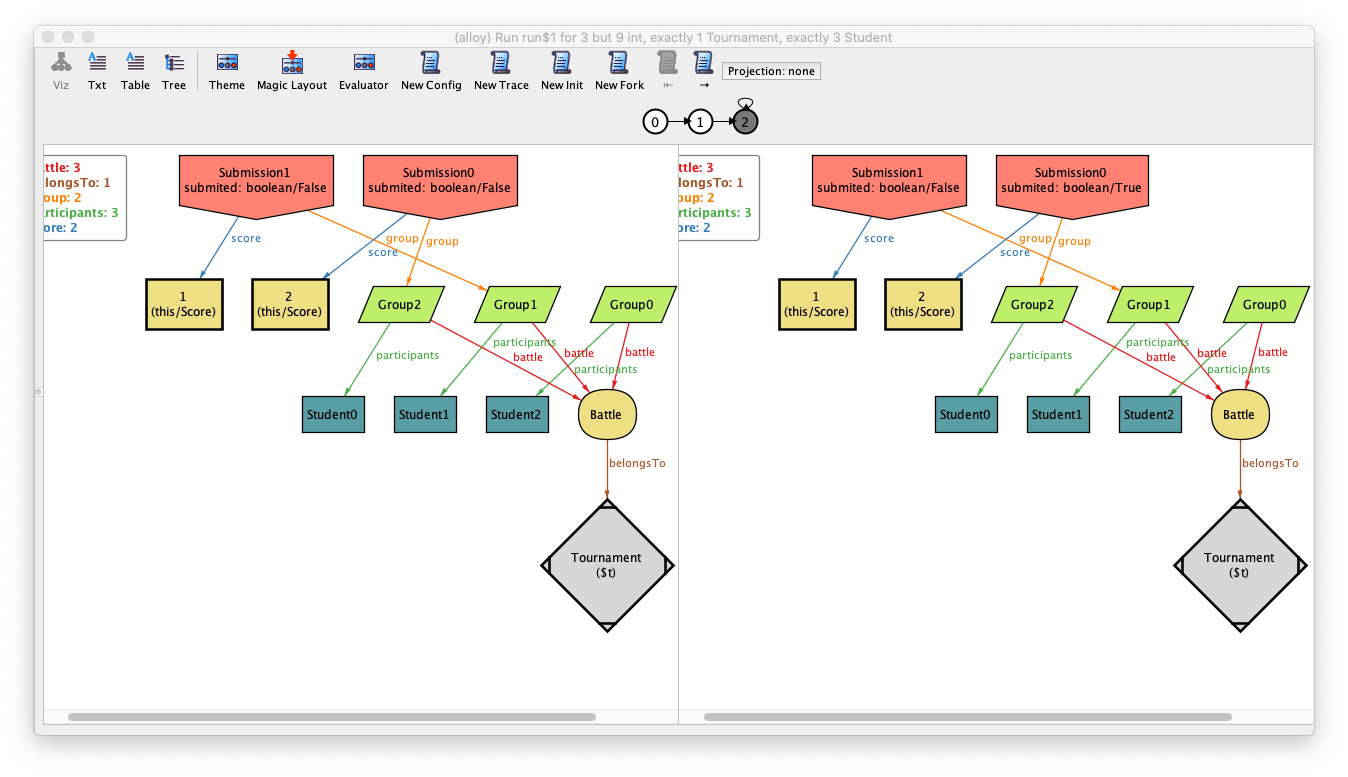
\includegraphics[width=\textwidth]{Images/Second example 1.png}
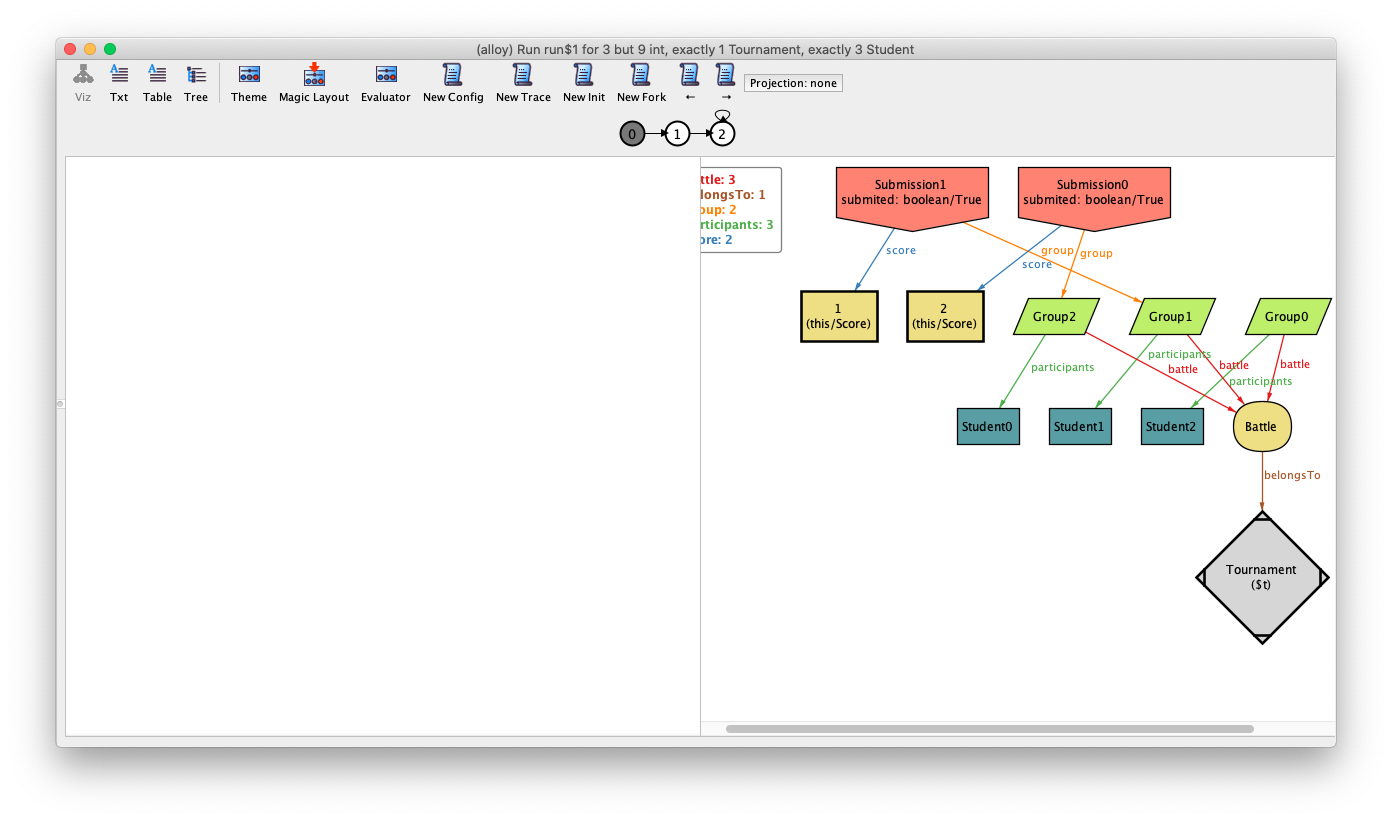
\includegraphics[width=\textwidth]{Images/Second example 2.png}
Final ranking:


\begin{tabular}{c|c}
    Student & Score \\
    \hline
    0 & 2 \\
    1 & 1 \\
    2 & 0 \\
\end{tabular}
\end{figure}


\begin{figure}[h]
\caption{Counterexample to prove that ranking is not always a partial order (neither a total order)  because of ties.}

\centering
\begin{lstlisting}[language=alloy]
check {
	after  all t:Tournament | partialOrder[t.ranking,t.participants]
}  for 9 Int
\end{lstlisting}

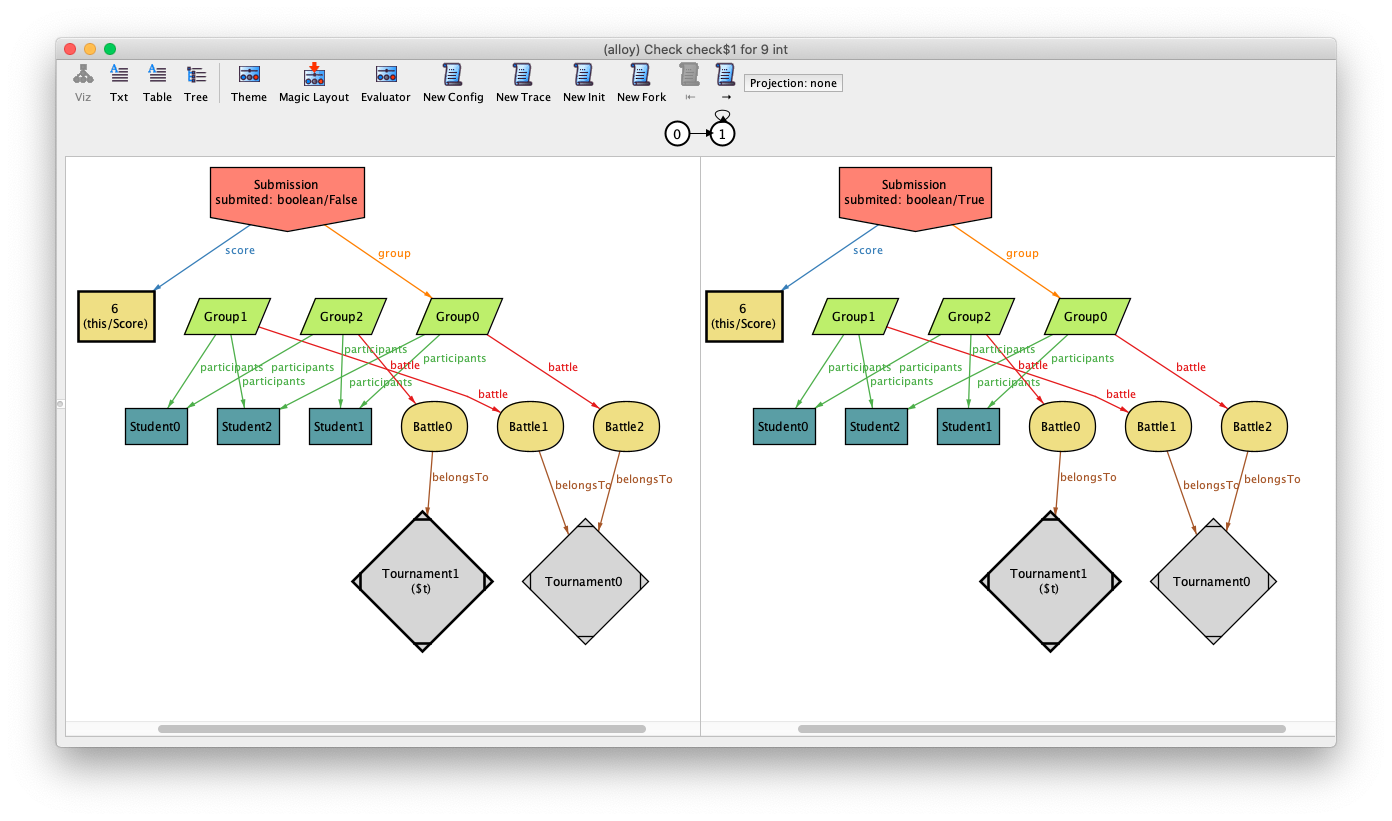
\includegraphics[width=\textwidth]{Images/Counterexample.png}
Final ranking for \$t:

\begin{tabular}{c|c}
    Student & Score \\
    \hline
    0 & 0 \\
    1 & 0 \\
\end{tabular}
\end{figure}

\begin{figure}[h]
\caption{Check that ranking is a preorder}

\centering
\begin{lstlisting}[language=alloy]
check {
	after all  t:Tournament |  preorder[t.ranking,t.participants]
} for 9 Int
\end{lstlisting}

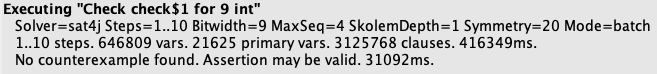
\includegraphics[width=\textwidth]{Images/Correct.png}
\end{figure}

\begin{figure}[h]
\caption{Simple example to show that a student can improve his score and tie the best one}

Because the relation has only 2 participants: the ranking relation is symmetric $\leftrightarrow$ there is a tie
\centering
\begin{lstlisting}[language=alloy]
run {
	eventually some  t:Tournament | #t.participants=2 and symmetric[t.ranking];
	some  t:Tournament | antisymmetric[t.ranking];
	some  t:Tournament | symmetric[t.ranking]
} for 3 but exactly 2 Student, 1 Tournament, 9 int
\end{lstlisting}

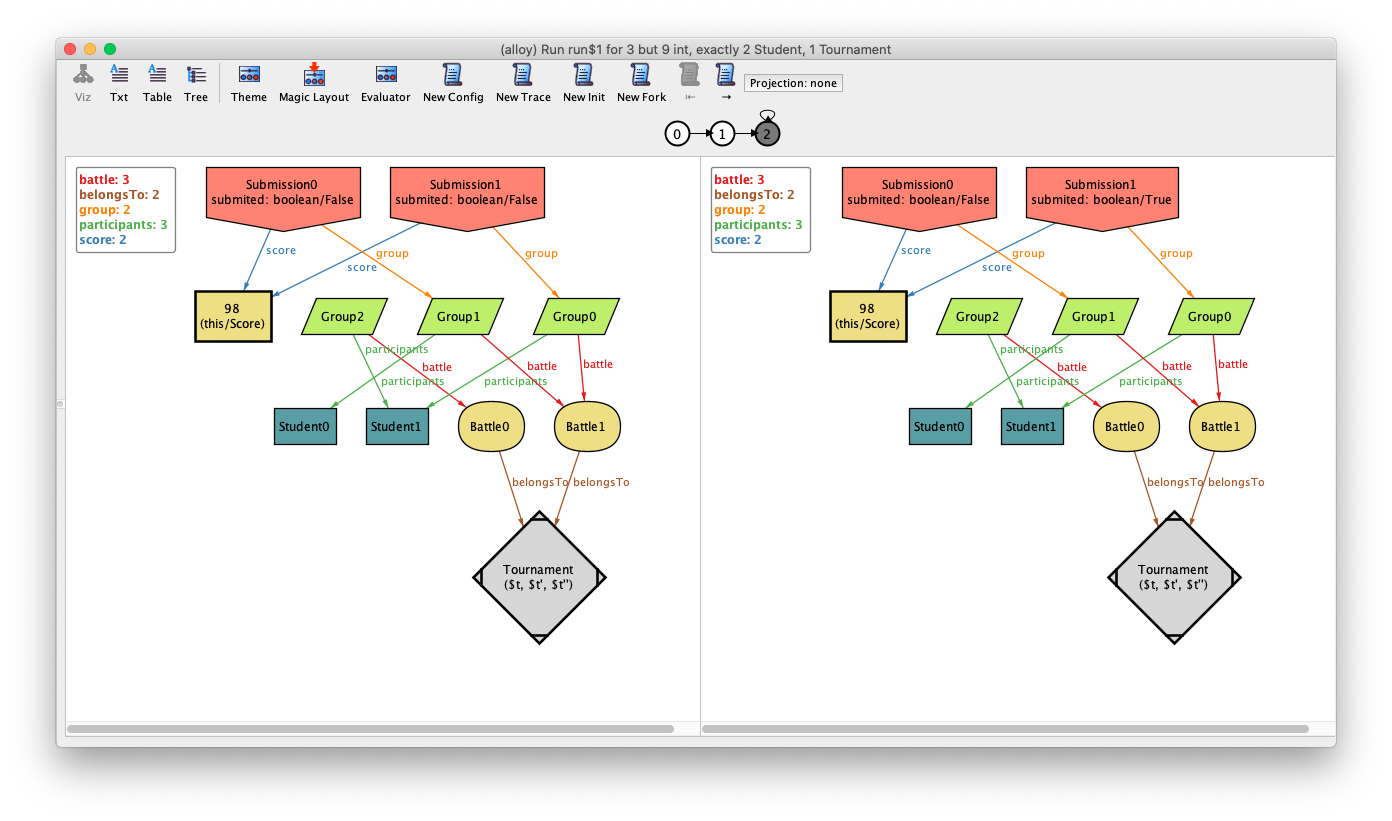
\includegraphics[width=\textwidth]{Images/Last example 1.png}
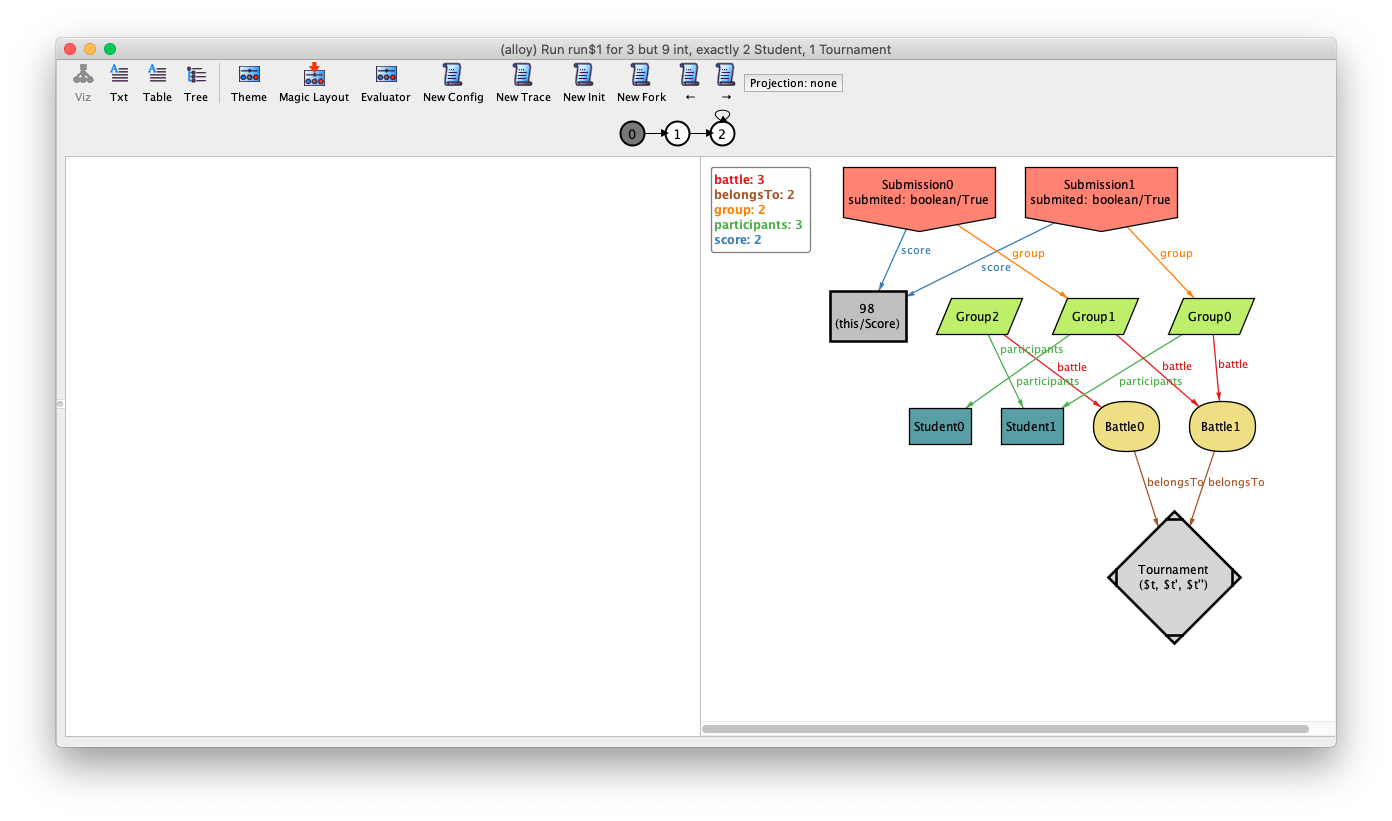
\includegraphics[width=\textwidth]{Images/Last example 2.png}
Ranking evolution:

\begin{tabular}{c||c|c|c}
    Student & Score & Score' & Score''\\
    \hline
    1 & 0 & 98 & 98\\
    0 & 0 & 0 & 98\\
\end{tabular}

\end{figure}